\chapter{Project Plan}

\section{Meetings}
Our goals were outlined by weekly meetings. We regularly met with Jacob Graff, our advisor throughout the development of Extend.
Jacob served as a sounding board whenever Extend's fundamental design philosophy was debated, and as a guide as we determined whether we were on track. We used any leftover time on those days to set goals for the upcoming week and pair program if time permitted.
\newline \newline
Our team also met weekly on Fridays to further discuss the progression of Extend. In the first half of the semester, the discussions were primarily philosophical, as decisions had to be made about the language grammar and behavior of certain Extend artifacts prior to development. In the second half, time was devoted to ironing out the development timeline, discussing bugs, and making compiler implementation decisions.

\section{Development Workflow}
  \begin{center}
  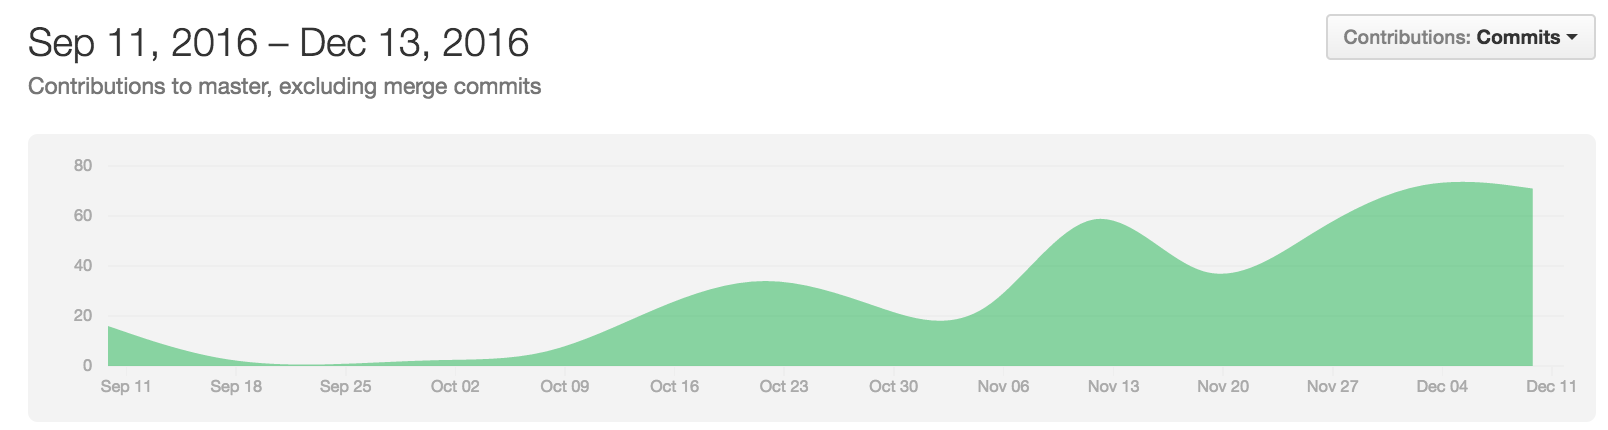
\includegraphics[width=.9\textwidth]{img/extend_git_graph.png}
  \end{center}

  \subsection{Github \& Travis CI}
  Our development and documentation were all done entirely through version control to maximize independent productivity.
  New features were introduced to the master branch through pull requests, and the team used this as a platform to peer review code to maximize code quality before such features entered production.

  \medskip \noindent
  An important aspect of development for us was continuous integration. Each pull request we made triggered a Travis build, which kept us informed regarding unexpected hiccups that sometimes arose during development. Travis CI ensured that new features were implemented with protecting the code base in mind, and provided quick visibility as to whether a new feature would break the existing build. Any changeset to the master branch must:

  \begin{enumerate}
    \item Pass Travis CI.
    \item Be approved by another member of the team.
    \item Be up to date with the master branch.
  \end{enumerate}

\section{Project Feature Completion Timeline}
Over the semester, we implemented our compiler from front end to back end, incorporating test cases throughout the way. Below are timestamps of our project progress throughout the semester.

  \begin{enumerate}
    \item Scanner (Early October)
    \item Parser and JSON output (Mid October)
    \item Finalize Language Semantics (Late October)
    \item Implement interpreter (Mostly feature complete by early November)
    \item Most transformations done, compile Hello World (Mid November)
    \item Finalize test suite (End November)
    \item Compile function calls, finish transformations (Early December)
    \item Compile references to variables (Early December)
    \item Feature complete compiler (December 15)
    \item Presentation to Professor Edwards (December 19)
  \end{enumerate}


\subsection{Style Guide}
  None of the team members had any prior experience with Ocaml. Fundamentally we were developing a certain style in the process of creating the project. A few style choices were clear soon after starting to develop in Ocaml:
  \begin{itemize}
  \item Avoid deep nesting of functions
  \item Instead build better abstraction and reuse functions
  \item Use \textbf{let ... in} instead of \textbf{and}. While this creates a lot of closures, it helped us to develop quicker by not needing to restructure code for changes
  \item Use underscore for values you won't use any further. Llvm code generation inherently creates a lot of values where the return value is of no use. Therefore mark those return values with an underscore, since it hides the warning.
  \item Indent with spaces, not tabs. Indent by 2 for each level of nesting.
  \item Make intentions clear by naming return values, not by naming LLVM indermediate values.
  \end{itemize}
These few rules helped us to control our code very well.\newline
Further we were developing our runtime in C. We applied the following style rules:
  \begin{itemize}
  \item Indent with tabs.
  \item Stick to C99.
  \item Use \textbf{value\_p} for user facing functions.
  \item Make sure to exit gracefully.
  \end{itemize}

\section{Language Evolution}
The language we delivered ended up surprisingly close to our initial proposal. The biggest change was to allow strings and ranges as value types, which made the language immeasurably better. Initially, we wanted to only have Numbers; but allowing cells to contain ranges (composite values) and not just primitive values makes it a much more useful language. Otherwise, the syntax and semantics are very close to what was in our original proposal.

Our initial plan was to precalculate the dependencies among cells as best as possible at compile time and generate code accordingly. However, it quickly became clear that the language was better with runtime-determined cell dependencies and we therefore had to give up on a precomputed graph. We didn't have time in this class to implement an explicit stack as opposed to using recursion, but this could be overcome if it had to be.

One minor change was to eliminate the dimension signature for functions. As we played around with the language in the interpreter, it became clear that we weren't using them and it wasn't obvious why we would; they were dropped as a result.


  \subsection{The Interpreter}
  Mainly because we implemented a declarative language, we built a working interpreter fairly early in the process to make sure we understood how to actually compile our language. Having it allowed us to test the language semantics, run example Extend programs, and make language decisions at an earlier stage. It also helped us benchmark the success of our compiler by comparing the number of testcases passed by both. A lot of the expressive power of Extend comes from the selection / slicing operator and a surprisingly high percentage of code in the compiler (20\% of the C runtime!) is devoted to handling selections. Having the details worked out in the interpreter gave us a road map that made the corresponding LLVM code generation much more straightforward. In addition, it was not obvious before having a working interpreter that we would need to have a scope (closure) object in order to allow recursion; if we had missed this important detail, we likely would have needed to make drastic code or language changes late in the process. Finally, it gave us confidence that the various transformations we performed on the source produced correct results.

\section{Team Member Responsibilities}

\begin{tabular}{ | l | l | l |}\hline
  Team Member  & Responsibilities      & GitHub Profile\\ \hline
  Jared Samet & design philosophy, semantic transformations, code generation  & \underline{\href{https://github.com/oracleofnj}{oracleofnj}}\\
  Nigel Schuster & development protocol, code generation, scripting  & \underline{\href{https://github.com/Neitsch}{Neitsch}}\\
  Ishaan Kolluri & initial LRM, Final Report, regression tests, stdlib functions, scripting & \underline{\href{https://github.com/ishaankolluri}{ishaankolluri}}\\
  Kevin Ye & initial scanner, regression tests, stdlib functions & \underline{\href{https://github.com/kevinye1}{kevinye1}}\\ \hline
\end{tabular}
